\documentclass[12pt,a4paper]{article}

\usepackage[a4paper,text={16.5cm,25.2cm},centering]{geometry}
\usepackage{lmodern}
\usepackage{amssymb,amsmath}
\usepackage{bm}
\usepackage{graphicx}
\usepackage{microtype}
\usepackage{hyperref}
\setlength{\parindent}{0pt}
\setlength{\parskip}{1.2ex}

\usepackage[makeroom]{cancel}

\usepackage{import}
\usepackage{pdfpages}
\usepackage{transparent}
\usepackage{xcolor}

\newcommand{\incfig}[2][1]{%
    \def\svgwidth{#1\columnwidth}
    \import{./figures/}{#2.pdf_tex}
}

\pdfsuppresswarningpagegroup=1
\hypersetup
       {   pdfauthor = { Kevin Corcoran },
           pdftitle={ HW \#5 Report},
           colorlinks=TRUE,
           linkcolor=black,
           citecolor=blue,
           urlcolor=blue
       }

\title{ HW \#5 Report}

\author{ Kevin Corcoran }


\usepackage{upquote}
\usepackage{listings}
\usepackage{xcolor}
\lstset{
    basicstyle=\ttfamily\footnotesize,
    upquote=true,
    breaklines=true,
    breakindent=0pt,
    keepspaces=true,
    showspaces=false,
    columns=fullflexible,
    showtabs=false,
    showstringspaces=false,
    escapeinside={(*@}{@*)},
    extendedchars=true,
}
\newcommand{\HLJLt}[1]{#1}
\newcommand{\HLJLw}[1]{#1}
\newcommand{\HLJLe}[1]{#1}
\newcommand{\HLJLeB}[1]{#1}
\newcommand{\HLJLo}[1]{#1}
\newcommand{\HLJLk}[1]{\textcolor[RGB]{148,91,176}{\textbf{#1}}}
\newcommand{\HLJLkc}[1]{\textcolor[RGB]{59,151,46}{\textit{#1}}}
\newcommand{\HLJLkd}[1]{\textcolor[RGB]{214,102,97}{\textit{#1}}}
\newcommand{\HLJLkn}[1]{\textcolor[RGB]{148,91,176}{\textbf{#1}}}
\newcommand{\HLJLkp}[1]{\textcolor[RGB]{148,91,176}{\textbf{#1}}}
\newcommand{\HLJLkr}[1]{\textcolor[RGB]{148,91,176}{\textbf{#1}}}
\newcommand{\HLJLkt}[1]{\textcolor[RGB]{148,91,176}{\textbf{#1}}}
\newcommand{\HLJLn}[1]{#1}
\newcommand{\HLJLna}[1]{#1}
\newcommand{\HLJLnb}[1]{#1}
\newcommand{\HLJLnbp}[1]{#1}
\newcommand{\HLJLnc}[1]{#1}
\newcommand{\HLJLncB}[1]{#1}
\newcommand{\HLJLnd}[1]{\textcolor[RGB]{214,102,97}{#1}}
\newcommand{\HLJLne}[1]{#1}
\newcommand{\HLJLneB}[1]{#1}
\newcommand{\HLJLnf}[1]{\textcolor[RGB]{66,102,213}{#1}}
\newcommand{\HLJLnfm}[1]{\textcolor[RGB]{66,102,213}{#1}}
\newcommand{\HLJLnp}[1]{#1}
\newcommand{\HLJLnl}[1]{#1}
\newcommand{\HLJLnn}[1]{#1}
\newcommand{\HLJLno}[1]{#1}
\newcommand{\HLJLnt}[1]{#1}
\newcommand{\HLJLnv}[1]{#1}
\newcommand{\HLJLnvc}[1]{#1}
\newcommand{\HLJLnvg}[1]{#1}
\newcommand{\HLJLnvi}[1]{#1}
\newcommand{\HLJLnvm}[1]{#1}
\newcommand{\HLJLl}[1]{#1}
\newcommand{\HLJLld}[1]{\textcolor[RGB]{148,91,176}{\textit{#1}}}
\newcommand{\HLJLs}[1]{\textcolor[RGB]{201,61,57}{#1}}
\newcommand{\HLJLsa}[1]{\textcolor[RGB]{201,61,57}{#1}}
\newcommand{\HLJLsb}[1]{\textcolor[RGB]{201,61,57}{#1}}
\newcommand{\HLJLsc}[1]{\textcolor[RGB]{201,61,57}{#1}}
\newcommand{\HLJLsd}[1]{\textcolor[RGB]{201,61,57}{#1}}
\newcommand{\HLJLsdB}[1]{\textcolor[RGB]{201,61,57}{#1}}
\newcommand{\HLJLsdC}[1]{\textcolor[RGB]{201,61,57}{#1}}
\newcommand{\HLJLse}[1]{\textcolor[RGB]{59,151,46}{#1}}
\newcommand{\HLJLsh}[1]{\textcolor[RGB]{201,61,57}{#1}}
\newcommand{\HLJLsi}[1]{#1}
\newcommand{\HLJLso}[1]{\textcolor[RGB]{201,61,57}{#1}}
\newcommand{\HLJLsr}[1]{\textcolor[RGB]{201,61,57}{#1}}
\newcommand{\HLJLss}[1]{\textcolor[RGB]{201,61,57}{#1}}
\newcommand{\HLJLssB}[1]{\textcolor[RGB]{201,61,57}{#1}}
\newcommand{\HLJLnB}[1]{\textcolor[RGB]{59,151,46}{#1}}
\newcommand{\HLJLnbB}[1]{\textcolor[RGB]{59,151,46}{#1}}
\newcommand{\HLJLnfB}[1]{\textcolor[RGB]{59,151,46}{#1}}
\newcommand{\HLJLnh}[1]{\textcolor[RGB]{59,151,46}{#1}}
\newcommand{\HLJLni}[1]{\textcolor[RGB]{59,151,46}{#1}}
\newcommand{\HLJLnil}[1]{\textcolor[RGB]{59,151,46}{#1}}
\newcommand{\HLJLnoB}[1]{\textcolor[RGB]{59,151,46}{#1}}
\newcommand{\HLJLoB}[1]{\textcolor[RGB]{102,102,102}{\textbf{#1}}}
\newcommand{\HLJLow}[1]{\textcolor[RGB]{102,102,102}{\textbf{#1}}}
\newcommand{\HLJLp}[1]{#1}
\newcommand{\HLJLc}[1]{\textcolor[RGB]{153,153,119}{\textit{#1}}}
\newcommand{\HLJLch}[1]{\textcolor[RGB]{153,153,119}{\textit{#1}}}
\newcommand{\HLJLcm}[1]{\textcolor[RGB]{153,153,119}{\textit{#1}}}
\newcommand{\HLJLcp}[1]{\textcolor[RGB]{153,153,119}{\textit{#1}}}
\newcommand{\HLJLcpB}[1]{\textcolor[RGB]{153,153,119}{\textit{#1}}}
\newcommand{\HLJLcs}[1]{\textcolor[RGB]{153,153,119}{\textit{#1}}}
\newcommand{\HLJLcsB}[1]{\textcolor[RGB]{153,153,119}{\textit{#1}}}
\newcommand{\HLJLg}[1]{#1}
\newcommand{\HLJLgd}[1]{#1}
\newcommand{\HLJLge}[1]{#1}
\newcommand{\HLJLgeB}[1]{#1}
\newcommand{\HLJLgh}[1]{#1}
\newcommand{\HLJLgi}[1]{#1}
\newcommand{\HLJLgo}[1]{#1}
\newcommand{\HLJLgp}[1]{#1}
\newcommand{\HLJLgs}[1]{#1}
\newcommand{\HLJLgsB}[1]{#1}
\newcommand{\HLJLgt}[1]{#1}


\begin{document}

\maketitle

\section{Problem 1}%
\label{sec:problem_1}

\subsection{Part 1}%
\label{sub:part_1}

\textbf{Carry out von Neumann stability analysis for the BTCS method} 

\vspace{15px}
\par Plug in $u_{i}^{n} = p^{n}e^{\sqrt{-1}\xi i\Delta x}$ to the BTCS method

\[
u_{i}^{n+1}=u_{i}^{n} + r \left(u_{i+1}^{n+1}-2u_{i}^{n+1}+u_{i-1}^{n+1}\right)
.\] 

\begin{align*}
  p^{n+1}e^{\sqrt{-1}\xi i\Delta x} &= p^{n}e^{\sqrt{-1}\xi i\Delta x}
  + r p^{n+1}e^{\sqrt{-1}\xi i\Delta x} \left(e^{\sqrt{-1}\xi\Delta x}
  - 2 + e^{-\sqrt{-1}\xi\Delta x} \right) \\
\end{align*}

\par Solving for $p$

\begin{align*}
  \left(e^{\sqrt{-1}\xi i\Delta x} -  r p^{n+1}e^{\sqrt{-1}\xi i\Delta x} \left(e^{\sqrt{-1}\xi\Delta x}
  - 2 + e^{-\sqrt{-1}\xi\Delta x}\right)\right) p^{n}p &= p^{n}e^{\sqrt{-1}\xi
i\Delta x} \\
\end{align*}

\begin{align*}
\implies p &= \frac{1}{1 - r \left(e^{\sqrt{-1}\xi \Delta x}
- 2 + e^{-\sqrt{-1}\xi \Delta x}\right)} \\
           &= \frac{1}{1 - 2r \left(\cos(\xi\Delta x) - 1\right) } \\
 &= \frac{1}{1 + 4r \left( \sin^2( \frac{\xi\Delta x}{2})\right) } 
\end{align*}


\vspace{15px}
\par We need $|p| \leq 1 + c\Delta t$. 
\vspace{15px}

Since $1 + 4r \left( \sin^2(
\frac{\xi\Delta x}{2})\right) \geq 1 \quad \forall\xi$

\[
\implies |p| = \left|\frac{1}{1 + 4r \left( \sin^2( \frac{\xi\Delta
x}{2})\right) } \right| \leq 1 + c\Delta t
.\] 

\vspace{15px}
\par so this method is unconditionally stable.

\section{Problem 2}%
\label{sec:problem_2}

\subsection{Part 1}%
\label{sub:part_1}

\textbf{Show $\lambda^{k} = 2(\cos(k\pi \Delta x) - 1)$ and $\omega^{k}
= \sin(k\pi i \Delta x) $are eigenvalues and eigenvectors of the matrix $(
\Delta x)^{2}A$.} 
\vspace{15px}

\par Consider the $i^{th}$ row of $A \omega^{k}$
\begin{align*}
  (A \omega^{k})_{i} &= \sin(k\pi(i-1)\Delta x) - 2\sin(k\pi i\Delta x)
  + \sin(k\pi (i+1)\Delta x) \\ 
                     &= \sin(k\pi i \Delta x - k\pi \Delta x) + \sin(k\pi
                     i \Delta x + k\pi\Delta x) - 2\sin(k\pi i \Delta x) \\
                     &= \sin(k\pi i \Delta x)\cos(k\pi \Delta x)
                     - \cancel{\cos(k\pi i \Delta x)\sin(k\pi \Delta x)}
                     + \sin(k\pi i \Delta x)\cos(k\pi \Delta x)
                     +\cancel{\cos(k\pi i \Delta x)\sin(k\pi \Delta x)}
                     - 2\sin(k\pi i \Delta x)\\
                     &=  \\
\end{align*}

This shows $2(\cos(k\pi \Delta x) - 1)$ is an eigenvalue and $\sin(k\pi
i \Delta x)$ is an eigenvector.


\subsection{Part 2}%
\label{sub:part_2}

Do the same for the vector $\cos(k\pi i \Delta x)$
\[
  \cos(k\pi(i-1)\Delta x) - 2\cos(k\pi i\Delta x) + \cos(k\pi(i+1) \Delta x)
.\] 

\subsection{Part 3}%
\label{sub:part_3}

We need zero boundary condition at $i=0$ and $i = N+1$.  $\cos(\dots i \dots)$ doesn't do that for us.


\section{Including required packages}

\begin{lstlisting}
(*@\HLJLk{using}@*) (*@\HLJLn{Plots}@*)
(*@\HLJLk{using}@*) (*@\HLJLn{LaTeXStrings}@*)
(*@\HLJLk{using}@*) (*@\HLJLn{SparseArrays}@*)
(*@\HLJLnf{theme}@*)(*@\HLJLp{(}@*)(*@\HLJLsc{:mute}@*)(*@\HLJLp{)}@*)

(*@\HLJLk{using}@*) (*@\HLJLn{Pkg}@*)
(*@\HLJLn{Pkg}@*)(*@\HLJLoB{.}@*)(*@\HLJLnf{activate}@*)(*@\HLJLp{(}@*)(*@\HLJLs{"{}DiffyQ"{}}@*)(*@\HLJLp{)}@*)
(*@\HLJLnf{include}@*)(*@\HLJLp{(}@*)(*@\HLJLs{"{}code/DiffyQ.jl"{}}@*)(*@\HLJLp{)}@*)
(*@\HLJLk{using}@*) (*@\HLJLoB{.}@*)(*@\HLJLn{DiffyQ}@*)(*@\HLJLoB{:}@*) (*@\HLJLn{ForwardEuler{\_}sys}@*)(*@\HLJLp{,}@*) (*@\HLJLn{Trapezoid{\_}sys}@*)(*@\HLJLp{,}@*) (*@\HLJLn{BTCS}@*)(*@\HLJLp{,}@*) (*@\HLJLn{s2{\_}DIRK{\_}sys}@*)(*@\HLJLp{,}@*) (*@\HLJLn{ForwardEuler{\_}tsys}@*)
\end{lstlisting}


\subsection{Setting up discretization for problems 3 and 4}

\begin{lstlisting}
(*@\HLJLcs{{\#}}@*) (*@\HLJLcs{Space}@*)
(*@\HLJLn{x0}@*) (*@\HLJLoB{=}@*) (*@\HLJLnfB{0.0}@*)(*@\HLJLp{;}@*) (*@\HLJLn{x}@*) (*@\HLJLoB{=}@*) (*@\HLJLnfB{2.0}@*)(*@\HLJLp{;}@*)
(*@\HLJLn{\ensuremath{\Delta}x}@*) (*@\HLJLoB{=}@*) (*@\HLJLnfB{0.01}@*)(*@\HLJLp{;}@*) (*@\HLJLn{L}@*) (*@\HLJLoB{=}@*) (*@\HLJLn{x}@*)(*@\HLJLoB{-}@*)(*@\HLJLn{x0}@*)(*@\HLJLp{;}@*) (*@\HLJLn{N}@*) (*@\HLJLoB{=}@*) (*@\HLJLnf{Int}@*)(*@\HLJLp{(}@*)(*@\HLJLn{L}@*)(*@\HLJLoB{/}@*)(*@\HLJLn{\ensuremath{\Delta}x}@*)(*@\HLJLp{);}@*) 

(*@\HLJLn{A}@*) (*@\HLJLoB{=}@*) (*@\HLJLni{1}@*)(*@\HLJLoB{/}@*)(*@\HLJLn{\ensuremath{\Delta}x}@*)(*@\HLJLoB{{\textasciicircum}}@*)(*@\HLJLni{2}@*) (*@\HLJLoB{*}@*) (*@\HLJLnf{spdiagm}@*)(*@\HLJLp{(}@*)(*@\HLJLoB{-}@*)(*@\HLJLni{1}@*)(*@\HLJLoB{=>}@*)(*@\HLJLnf{ones}@*)(*@\HLJLp{(}@*)(*@\HLJLn{N}@*)(*@\HLJLoB{-}@*)(*@\HLJLni{1}@*)(*@\HLJLp{),}@*)(*@\HLJLni{0}@*)(*@\HLJLoB{=>-}@*)(*@\HLJLnfB{2.0}@*)(*@\HLJLoB{*}@*)(*@\HLJLnf{ones}@*)(*@\HLJLp{(}@*)(*@\HLJLn{N}@*)(*@\HLJLp{),}@*)(*@\HLJLni{1}@*)(*@\HLJLoB{=>}@*)(*@\HLJLnf{ones}@*)(*@\HLJLp{(}@*)(*@\HLJLn{N}@*)(*@\HLJLoB{-}@*)(*@\HLJLni{1}@*)(*@\HLJLp{))}@*)

(*@\HLJLcs{{\#}}@*) (*@\HLJLcs{Time}@*)
(*@\HLJLn{t0}@*) (*@\HLJLoB{=}@*) (*@\HLJLnfB{0.0}@*)(*@\HLJLp{;}@*) (*@\HLJLn{t}@*) (*@\HLJLoB{=}@*) (*@\HLJLnfB{0.2}@*)(*@\HLJLp{;}@*) 
(*@\HLJLn{T}@*) (*@\HLJLoB{=}@*) (*@\HLJLn{t}@*)(*@\HLJLoB{-}@*)(*@\HLJLn{t0}@*)(*@\HLJLp{;}@*)
\end{lstlisting}


\section{Problem 3:}
\subsection{Stable threshold}

\begin{lstlisting}
(*@\HLJLcs{{\#}}@*) (*@\HLJLcs{\ensuremath{\Delta}t}@*) (*@\HLJLcs{=}@*) (*@\HLJLcs{(\ensuremath{\Delta}x){\textasciicircum}2/2}@*) (*@\HLJLcs{*}@*) (*@\HLJLcs{1/0.99;}@*) (*@\HLJLcs{M}@*) (*@\HLJLcs{=}@*) (*@\HLJLcs{Int(T/\ensuremath{\Delta}t);}@*) (*@\HLJLcs{{\#}}@*) (*@\HLJLcs{unstable}@*)
(*@\HLJLn{\ensuremath{\Delta}t}@*) (*@\HLJLoB{=}@*) (*@\HLJLp{(}@*)(*@\HLJLn{\ensuremath{\Delta}x}@*)(*@\HLJLp{)}@*)(*@\HLJLoB{{\textasciicircum}}@*)(*@\HLJLni{2}@*)(*@\HLJLoB{/}@*)(*@\HLJLni{2}@*) (*@\HLJLoB{*}@*) (*@\HLJLni{1}@*)(*@\HLJLoB{/}@*)(*@\HLJLnfB{1.01}@*)(*@\HLJLp{;}@*) (*@\HLJLn{M}@*) (*@\HLJLoB{=}@*) (*@\HLJLnf{Int}@*)(*@\HLJLp{(}@*)(*@\HLJLn{T}@*)(*@\HLJLoB{/}@*)(*@\HLJLn{\ensuremath{\Delta}t}@*)(*@\HLJLp{);}@*) (*@\HLJLcs{{\#}}@*) (*@\HLJLcs{stable}@*)

(*@\HLJLcs{{\#}}@*) (*@\HLJLcs{initial}@*) (*@\HLJLcs{condition}@*)
(*@\HLJLnf{f}@*)(*@\HLJLp{(}@*)(*@\HLJLn{x}@*)(*@\HLJLp{)}@*) (*@\HLJLoB{=}@*) (*@\HLJLnf{convert}@*)(*@\HLJLp{(}@*)(*@\HLJLnf{Array}@*)(*@\HLJLp{{\{}}@*)(*@\HLJLn{Float64}@*)(*@\HLJLp{{\}},}@*) (*@\HLJLp{(}@*)(*@\HLJLn{x}@*) (*@\HLJLoB{.<}@*) (*@\HLJLni{1}@*)(*@\HLJLp{)}@*) (*@\HLJLoB{.{\&}}@*) (*@\HLJLp{(}@*)(*@\HLJLn{x}@*) (*@\HLJLoB{.>}@*) (*@\HLJLni{0}@*)(*@\HLJLp{))}@*)

(*@\HLJLcs{{\#}}@*) (*@\HLJLcs{boundary}@*) (*@\HLJLcs{condition}@*)
(*@\HLJLn{b}@*) (*@\HLJLoB{=}@*) (*@\HLJLnf{zeros}@*)(*@\HLJLp{(}@*)(*@\HLJLn{N}@*)(*@\HLJLp{);}@*) (*@\HLJLn{b}@*)(*@\HLJLp{[}@*)(*@\HLJLni{1}@*)(*@\HLJLp{]}@*) (*@\HLJLoB{=}@*) (*@\HLJLnfB{1.0}@*)(*@\HLJLp{;}@*) (*@\HLJLn{b}@*)(*@\HLJLp{[}@*)(*@\HLJLk{end}@*)(*@\HLJLp{]}@*) (*@\HLJLoB{=}@*) (*@\HLJLnfB{0.0}@*)(*@\HLJLp{;}@*) (*@\HLJLn{b}@*) (*@\HLJLoB{=}@*) (*@\HLJLni{1}@*)(*@\HLJLoB{/}@*)(*@\HLJLp{(}@*)(*@\HLJLn{\ensuremath{\Delta}x}@*)(*@\HLJLoB{{\textasciicircum}}@*)(*@\HLJLni{2}@*)(*@\HLJLp{)}@*) (*@\HLJLoB{*}@*) (*@\HLJLn{b}@*)(*@\HLJLp{;}@*)

(*@\HLJLn{xs}@*) (*@\HLJLoB{=}@*) (*@\HLJLnf{collect}@*)(*@\HLJLp{(}@*)(*@\HLJLni{0}@*)(*@\HLJLoB{:}@*)(*@\HLJLn{N}@*)(*@\HLJLoB{-}@*)(*@\HLJLni{1}@*)(*@\HLJLp{)}@*)(*@\HLJLoB{*}@*)(*@\HLJLn{\ensuremath{\Delta}x}@*)
(*@\HLJLn{u0}@*) (*@\HLJLoB{=}@*) (*@\HLJLnf{f}@*)(*@\HLJLp{(}@*)(*@\HLJLn{xs}@*)(*@\HLJLp{)}@*)

(*@\HLJLn{u}@*) (*@\HLJLoB{=}@*) (*@\HLJLnf{ForwardEuler{\_}sys}@*)(*@\HLJLp{(}@*)(*@\HLJLn{M}@*)(*@\HLJLp{,}@*) (*@\HLJLn{T}@*)(*@\HLJLp{,}@*) (*@\HLJLn{u0}@*)(*@\HLJLp{,}@*) (*@\HLJLn{A}@*)(*@\HLJLp{,}@*) (*@\HLJLn{b}@*)(*@\HLJLp{)}@*)

(*@\HLJLn{xs}@*) (*@\HLJLoB{=}@*) (*@\HLJLnf{collect}@*)(*@\HLJLp{(}@*)(*@\HLJLni{0}@*)(*@\HLJLoB{:}@*)(*@\HLJLn{N}@*)(*@\HLJLp{)}@*)(*@\HLJLoB{*}@*)(*@\HLJLn{\ensuremath{\Delta}x}@*)

(*@\HLJLn{ts}@*) (*@\HLJLoB{=}@*) (*@\HLJLp{(}@*)(*@\HLJLni{1}@*)(*@\HLJLoB{:}@*)(*@\HLJLni{3}@*)(*@\HLJLp{)}@*) (*@\HLJLoB{.{\textasciicircum}}@*)(*@\HLJLni{2}@*) (*@\HLJLoB{*}@*) (*@\HLJLnfB{1e-2}@*)
(*@\HLJLn{ms}@*) (*@\HLJLoB{=}@*) (*@\HLJLn{Int}@*)(*@\HLJLoB{.}@*)(*@\HLJLp{(}@*)(*@\HLJLn{floor}@*)(*@\HLJLoB{.}@*)(*@\HLJLp{((}@*)(*@\HLJLn{ts}@*) (*@\HLJLoB{.-}@*) (*@\HLJLn{t0}@*)(*@\HLJLp{)}@*)(*@\HLJLoB{/}@*)(*@\HLJLn{\ensuremath{\Delta}t}@*)(*@\HLJLp{))}@*)(*@\HLJLcs{{\#}}@*) (*@\HLJLcs{indices}@*) (*@\HLJLcs{for}@*) (*@\HLJLcs{ts}@*)
(*@\HLJLnf{plot}@*)(*@\HLJLp{(}@*)(*@\HLJLn{xs}@*)(*@\HLJLp{[}@*)(*@\HLJLni{1}@*)(*@\HLJLoB{:}@*)(*@\HLJLn{N}@*)(*@\HLJLp{],}@*) (*@\HLJLn{u0}@*)(*@\HLJLp{[}@*)(*@\HLJLni{1}@*)(*@\HLJLoB{:}@*)(*@\HLJLn{N}@*)(*@\HLJLp{],}@*) (*@\HLJLn{label}@*) (*@\HLJLoB{=}@*) (*@\HLJLnf{latexstring}@*)(*@\HLJLp{(}@*)(*@\HLJLs{"{}t}@*) (*@\HLJLs{=}@*) (*@\HLJLs{"{}}@*)(*@\HLJLp{,}@*) (*@\HLJLni{0}@*) (*@\HLJLp{))}@*)
(*@\HLJLn{j}@*) (*@\HLJLoB{=}@*) (*@\HLJLni{1}@*)
(*@\HLJLk{for}@*) (*@\HLJLn{i}@*) (*@\HLJLoB{\ensuremath{\in}}@*) (*@\HLJLn{ms}@*)
    (*@\HLJLnf{plot!}@*)(*@\HLJLp{(}@*)(*@\HLJLn{xs}@*)(*@\HLJLp{[}@*)(*@\HLJLni{1}@*)(*@\HLJLoB{:}@*)(*@\HLJLn{N}@*)(*@\HLJLp{],}@*) (*@\HLJLn{u}@*)(*@\HLJLp{[}@*)(*@\HLJLni{1}@*)(*@\HLJLoB{:}@*)(*@\HLJLn{N}@*)(*@\HLJLp{,}@*) (*@\HLJLn{i}@*)(*@\HLJLp{],}@*) (*@\HLJLn{label}@*) (*@\HLJLoB{=}@*) (*@\HLJLnf{latexstring}@*)(*@\HLJLp{(}@*)(*@\HLJLs{"{}t}@*) (*@\HLJLs{=}@*) (*@\HLJLs{"{}}@*)(*@\HLJLp{,}@*)(*@\HLJLn{ts}@*)(*@\HLJLp{[}@*)(*@\HLJLn{j}@*)(*@\HLJLp{]))}@*)
    (*@\HLJLkd{global}@*) (*@\HLJLn{j}@*) (*@\HLJLoB{=}@*) (*@\HLJLn{j}@*) (*@\HLJLoB{+}@*) (*@\HLJLni{1}@*)
(*@\HLJLk{end}@*)

(*@\HLJLnf{plot!}@*)(*@\HLJLp{(}@*)(*@\HLJLn{xs}@*)(*@\HLJLp{[}@*)(*@\HLJLni{1}@*)(*@\HLJLoB{:}@*)(*@\HLJLn{N}@*)(*@\HLJLp{],}@*) (*@\HLJLn{u}@*)(*@\HLJLp{[}@*)(*@\HLJLni{1}@*)(*@\HLJLoB{:}@*)(*@\HLJLn{N}@*)(*@\HLJLp{,}@*) (*@\HLJLk{end}@*)(*@\HLJLp{],}@*) (*@\HLJLn{label}@*) (*@\HLJLoB{=}@*) (*@\HLJLnf{latexstring}@*)(*@\HLJLp{(}@*)(*@\HLJLs{"{}t}@*) (*@\HLJLs{=}@*) (*@\HLJLs{"{}}@*)(*@\HLJLp{,}@*) (*@\HLJLnfB{0.2}@*)(*@\HLJLp{))}@*)
\end{lstlisting}

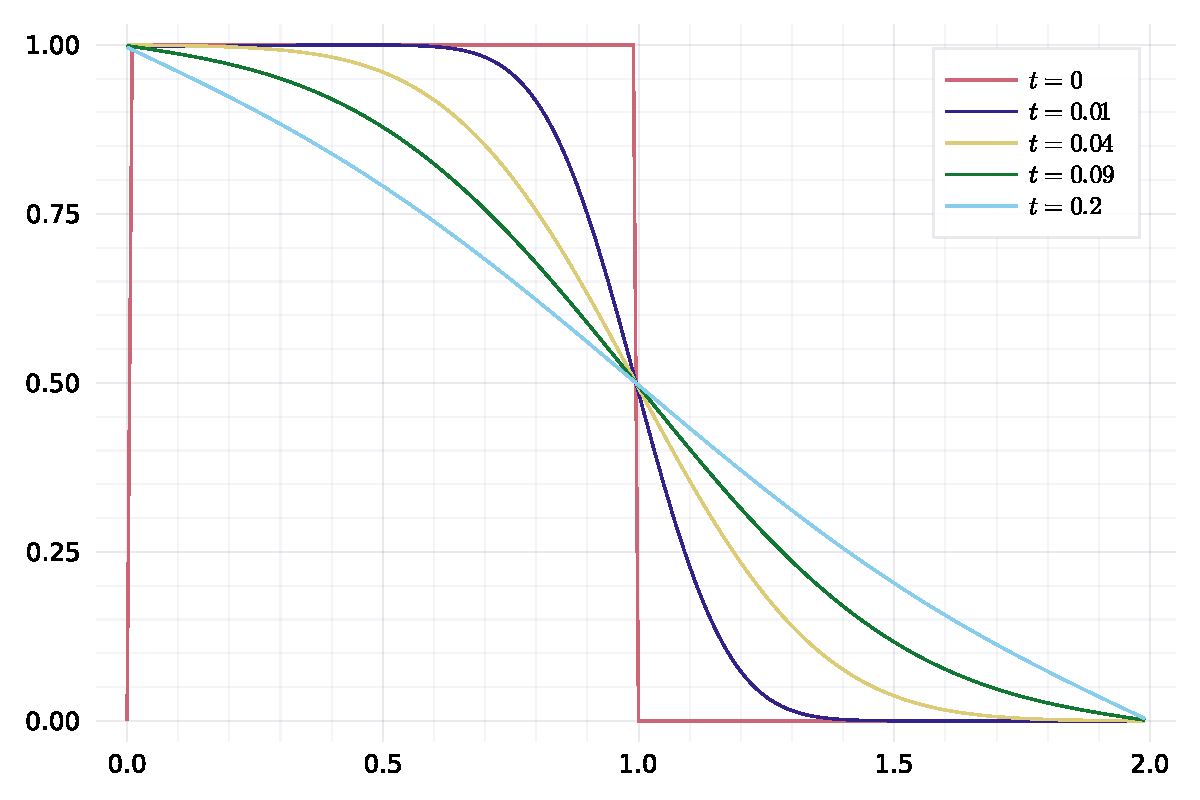
\includegraphics[width=\linewidth]{figures/ass_5_report_3_1.pdf}

\subsection{Unstable threshold}

\begin{lstlisting}
(*@\HLJLn{\ensuremath{\Delta}t}@*) (*@\HLJLoB{=}@*) (*@\HLJLp{(}@*)(*@\HLJLn{\ensuremath{\Delta}x}@*)(*@\HLJLp{)}@*)(*@\HLJLoB{{\textasciicircum}}@*)(*@\HLJLni{2}@*)(*@\HLJLoB{/}@*)(*@\HLJLni{2}@*) (*@\HLJLoB{*}@*) (*@\HLJLni{1}@*)(*@\HLJLoB{/}@*)(*@\HLJLnfB{0.99}@*)(*@\HLJLp{;}@*) (*@\HLJLn{M}@*) (*@\HLJLoB{=}@*) (*@\HLJLnf{Int}@*)(*@\HLJLp{(}@*)(*@\HLJLn{T}@*)(*@\HLJLoB{/}@*)(*@\HLJLn{\ensuremath{\Delta}t}@*)(*@\HLJLp{);}@*) (*@\HLJLcs{{\#}}@*) (*@\HLJLcs{unstable}@*)

(*@\HLJLcs{{\#}}@*) (*@\HLJLcs{initial}@*) (*@\HLJLcs{condition}@*)
(*@\HLJLnf{f}@*)(*@\HLJLp{(}@*)(*@\HLJLn{x}@*)(*@\HLJLp{)}@*) (*@\HLJLoB{=}@*) (*@\HLJLnf{convert}@*)(*@\HLJLp{(}@*)(*@\HLJLnf{Array}@*)(*@\HLJLp{{\{}}@*)(*@\HLJLn{Float64}@*)(*@\HLJLp{{\}},}@*) (*@\HLJLp{(}@*)(*@\HLJLn{x}@*) (*@\HLJLoB{.<}@*) (*@\HLJLni{1}@*)(*@\HLJLp{)}@*) (*@\HLJLoB{.{\&}}@*) (*@\HLJLp{(}@*)(*@\HLJLn{x}@*) (*@\HLJLoB{.>}@*) (*@\HLJLni{0}@*)(*@\HLJLp{))}@*)

(*@\HLJLcs{{\#}}@*) (*@\HLJLcs{boundary}@*) (*@\HLJLcs{condition}@*)
(*@\HLJLn{b}@*) (*@\HLJLoB{=}@*) (*@\HLJLnf{zeros}@*)(*@\HLJLp{(}@*)(*@\HLJLn{N}@*)(*@\HLJLp{);}@*) (*@\HLJLn{b}@*)(*@\HLJLp{[}@*)(*@\HLJLni{1}@*)(*@\HLJLp{]}@*) (*@\HLJLoB{=}@*) (*@\HLJLnfB{1.0}@*)(*@\HLJLp{;}@*) (*@\HLJLn{b}@*)(*@\HLJLp{[}@*)(*@\HLJLk{end}@*)(*@\HLJLp{]}@*) (*@\HLJLoB{=}@*) (*@\HLJLnfB{0.0}@*)(*@\HLJLp{;}@*) (*@\HLJLn{b}@*) (*@\HLJLoB{=}@*) (*@\HLJLni{1}@*)(*@\HLJLoB{/}@*)(*@\HLJLp{(}@*)(*@\HLJLn{\ensuremath{\Delta}x}@*)(*@\HLJLoB{{\textasciicircum}}@*)(*@\HLJLni{2}@*)(*@\HLJLp{)}@*) (*@\HLJLoB{*}@*) (*@\HLJLn{b}@*)(*@\HLJLp{;}@*)

(*@\HLJLn{xs}@*) (*@\HLJLoB{=}@*) (*@\HLJLnf{collect}@*)(*@\HLJLp{(}@*)(*@\HLJLni{0}@*)(*@\HLJLoB{:}@*)(*@\HLJLn{N}@*)(*@\HLJLoB{-}@*)(*@\HLJLni{1}@*)(*@\HLJLp{)}@*)(*@\HLJLoB{*}@*)(*@\HLJLn{\ensuremath{\Delta}x}@*)
(*@\HLJLn{u0}@*) (*@\HLJLoB{=}@*) (*@\HLJLnf{f}@*)(*@\HLJLp{(}@*)(*@\HLJLn{xs}@*)(*@\HLJLp{)}@*)

(*@\HLJLn{u}@*) (*@\HLJLoB{=}@*) (*@\HLJLnf{ForwardEuler{\_}sys}@*)(*@\HLJLp{(}@*)(*@\HLJLn{M}@*)(*@\HLJLp{,}@*) (*@\HLJLn{T}@*)(*@\HLJLp{,}@*) (*@\HLJLn{u0}@*)(*@\HLJLp{,}@*) (*@\HLJLn{A}@*)(*@\HLJLp{,}@*) (*@\HLJLn{b}@*)(*@\HLJLp{)}@*)

(*@\HLJLn{xs}@*) (*@\HLJLoB{=}@*) (*@\HLJLnf{collect}@*)(*@\HLJLp{(}@*)(*@\HLJLni{0}@*)(*@\HLJLoB{:}@*)(*@\HLJLn{N}@*)(*@\HLJLp{)}@*)(*@\HLJLoB{*}@*)(*@\HLJLn{\ensuremath{\Delta}x}@*)

(*@\HLJLn{ts}@*) (*@\HLJLoB{=}@*) (*@\HLJLp{(}@*)(*@\HLJLni{1}@*)(*@\HLJLoB{:}@*)(*@\HLJLni{3}@*)(*@\HLJLp{)}@*) (*@\HLJLoB{.{\textasciicircum}}@*)(*@\HLJLni{2}@*) (*@\HLJLoB{*}@*) (*@\HLJLnfB{1e-2}@*)
(*@\HLJLn{ms}@*) (*@\HLJLoB{=}@*) (*@\HLJLn{Int}@*)(*@\HLJLoB{.}@*)(*@\HLJLp{(}@*)(*@\HLJLn{floor}@*)(*@\HLJLoB{.}@*)(*@\HLJLp{((}@*)(*@\HLJLn{ts}@*) (*@\HLJLoB{.-}@*) (*@\HLJLn{t0}@*)(*@\HLJLp{)}@*)(*@\HLJLoB{/}@*)(*@\HLJLn{\ensuremath{\Delta}t}@*)(*@\HLJLp{))}@*)(*@\HLJLcs{{\#}}@*) (*@\HLJLcs{indices}@*) (*@\HLJLcs{for}@*) (*@\HLJLcs{ts}@*)
(*@\HLJLnf{plot}@*)(*@\HLJLp{(}@*)(*@\HLJLn{xs}@*)(*@\HLJLp{[}@*)(*@\HLJLni{1}@*)(*@\HLJLoB{:}@*)(*@\HLJLn{N}@*)(*@\HLJLp{],}@*) (*@\HLJLn{u0}@*)(*@\HLJLp{[}@*)(*@\HLJLni{1}@*)(*@\HLJLoB{:}@*)(*@\HLJLn{N}@*)(*@\HLJLp{],}@*) (*@\HLJLn{label}@*) (*@\HLJLoB{=}@*) (*@\HLJLnf{latexstring}@*)(*@\HLJLp{(}@*)(*@\HLJLs{"{}t}@*) (*@\HLJLs{=}@*) (*@\HLJLs{"{}}@*)(*@\HLJLp{,}@*) (*@\HLJLni{0}@*) (*@\HLJLp{))}@*)
(*@\HLJLn{j}@*) (*@\HLJLoB{=}@*) (*@\HLJLni{1}@*)
(*@\HLJLk{for}@*) (*@\HLJLn{i}@*) (*@\HLJLoB{\ensuremath{\in}}@*) (*@\HLJLn{ms}@*)
    (*@\HLJLnf{plot!}@*)(*@\HLJLp{(}@*)(*@\HLJLn{xs}@*)(*@\HLJLp{[}@*)(*@\HLJLni{1}@*)(*@\HLJLoB{:}@*)(*@\HLJLn{N}@*)(*@\HLJLp{],}@*) (*@\HLJLn{u}@*)(*@\HLJLp{[}@*)(*@\HLJLni{1}@*)(*@\HLJLoB{:}@*)(*@\HLJLn{N}@*)(*@\HLJLp{,}@*) (*@\HLJLn{i}@*)(*@\HLJLp{],}@*) (*@\HLJLn{label}@*) (*@\HLJLoB{=}@*) (*@\HLJLnf{latexstring}@*)(*@\HLJLp{(}@*)(*@\HLJLs{"{}t}@*) (*@\HLJLs{=}@*) (*@\HLJLs{"{}}@*)(*@\HLJLp{,}@*)(*@\HLJLn{ts}@*)(*@\HLJLp{[}@*)(*@\HLJLn{j}@*)(*@\HLJLp{]))}@*)
    (*@\HLJLkd{global}@*) (*@\HLJLn{j}@*) (*@\HLJLoB{=}@*) (*@\HLJLn{j}@*) (*@\HLJLoB{+}@*) (*@\HLJLni{1}@*)
(*@\HLJLk{end}@*)

(*@\HLJLnf{plot!}@*)(*@\HLJLp{(}@*)(*@\HLJLn{xs}@*)(*@\HLJLp{[}@*)(*@\HLJLni{1}@*)(*@\HLJLoB{:}@*)(*@\HLJLn{N}@*)(*@\HLJLp{],}@*) (*@\HLJLn{u}@*)(*@\HLJLp{[}@*)(*@\HLJLni{1}@*)(*@\HLJLoB{:}@*)(*@\HLJLn{N}@*)(*@\HLJLp{,}@*) (*@\HLJLk{end}@*)(*@\HLJLp{],}@*) (*@\HLJLn{label}@*) (*@\HLJLoB{=}@*) (*@\HLJLnf{latexstring}@*)(*@\HLJLp{(}@*)(*@\HLJLs{"{}t}@*) (*@\HLJLs{=}@*) (*@\HLJLs{"{}}@*)(*@\HLJLp{,}@*) (*@\HLJLnfB{0.2}@*)(*@\HLJLp{))}@*)
\end{lstlisting}

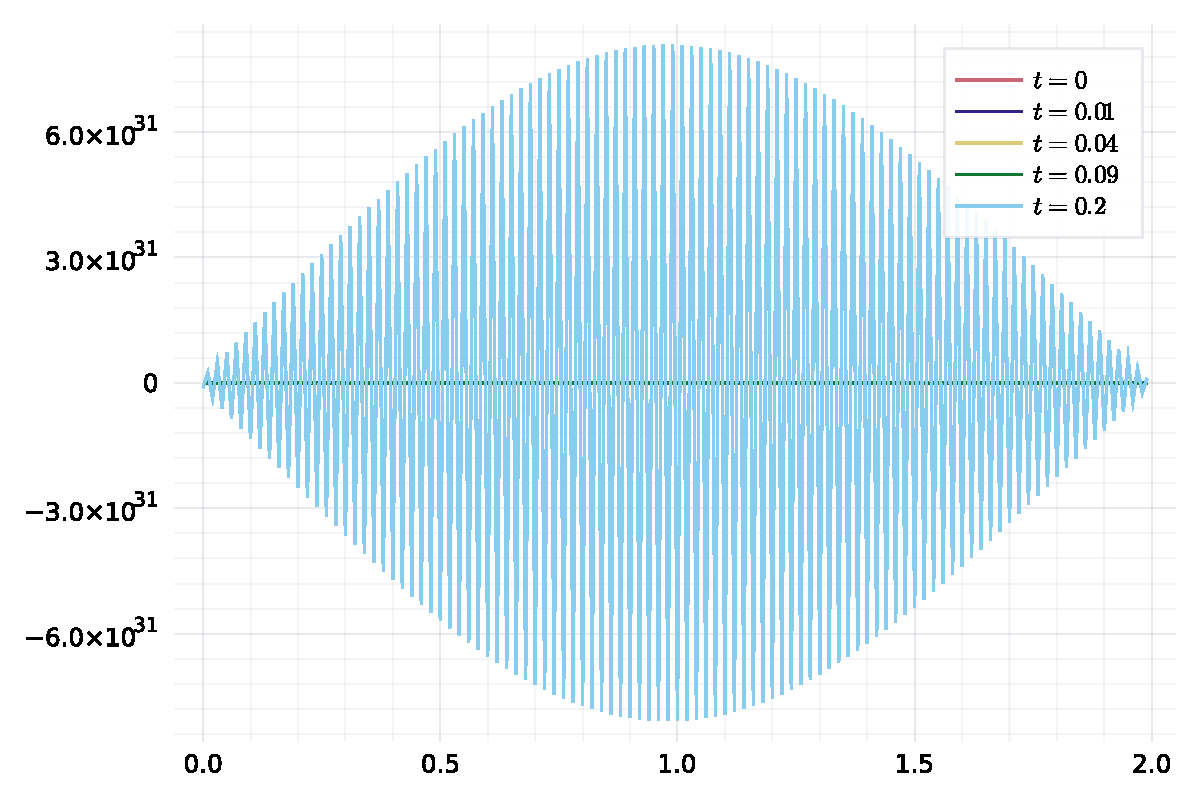
\includegraphics[width=\linewidth]{figures/ass_5_report_4_1.pdf}

\section{Problem 4:}
\subsection{BTCS (Backward Euler)}

\begin{lstlisting}
(*@\HLJLn{\ensuremath{\Delta}t}@*) (*@\HLJLoB{=}@*) (*@\HLJLnfB{0.01}@*)(*@\HLJLp{;}@*) (*@\HLJLn{M}@*) (*@\HLJLoB{=}@*) (*@\HLJLnf{Int}@*)(*@\HLJLp{(}@*)(*@\HLJLn{T}@*)(*@\HLJLoB{/}@*)(*@\HLJLn{\ensuremath{\Delta}t}@*)(*@\HLJLp{);}@*)
(*@\HLJLcs{{\#}}@*) (*@\HLJLcs{Backward}@*) (*@\HLJLcs{Euler}@*)
(*@\HLJLn{u}@*) (*@\HLJLoB{=}@*) (*@\HLJLnf{BTCS}@*)(*@\HLJLp{(}@*)(*@\HLJLn{M}@*)(*@\HLJLp{,}@*) (*@\HLJLn{T}@*)(*@\HLJLp{,}@*) (*@\HLJLn{u0}@*)(*@\HLJLp{,}@*) (*@\HLJLn{A}@*)(*@\HLJLp{,}@*) (*@\HLJLn{b}@*)(*@\HLJLp{)}@*)

(*@\HLJLcs{{\#}}@*) (*@\HLJLcs{Plotting}@*) (*@\HLJLcs{routine}@*)
(*@\HLJLn{ts}@*) (*@\HLJLoB{=}@*) (*@\HLJLp{(}@*)(*@\HLJLni{1}@*)(*@\HLJLoB{:}@*)(*@\HLJLni{3}@*)(*@\HLJLp{)}@*) (*@\HLJLoB{.{\textasciicircum}}@*)(*@\HLJLni{2}@*) (*@\HLJLoB{*}@*) (*@\HLJLnfB{1e-2}@*)
(*@\HLJLn{ms}@*) (*@\HLJLoB{=}@*) (*@\HLJLn{Int}@*)(*@\HLJLoB{.}@*)(*@\HLJLp{(}@*)(*@\HLJLn{floor}@*)(*@\HLJLoB{.}@*)(*@\HLJLp{((}@*)(*@\HLJLn{ts}@*) (*@\HLJLoB{.-}@*) (*@\HLJLn{t0}@*)(*@\HLJLp{)}@*)(*@\HLJLoB{/}@*)(*@\HLJLn{\ensuremath{\Delta}t}@*)(*@\HLJLp{))}@*)(*@\HLJLcs{{\#}}@*) (*@\HLJLcs{indices}@*) (*@\HLJLcs{for}@*) (*@\HLJLcs{ts}@*)
(*@\HLJLnf{plot}@*)(*@\HLJLp{(}@*)(*@\HLJLn{xs}@*)(*@\HLJLp{[}@*)(*@\HLJLni{1}@*)(*@\HLJLoB{:}@*)(*@\HLJLn{N}@*)(*@\HLJLp{],}@*) (*@\HLJLn{u0}@*)(*@\HLJLp{[}@*)(*@\HLJLni{1}@*)(*@\HLJLoB{:}@*)(*@\HLJLn{N}@*)(*@\HLJLp{],}@*) (*@\HLJLn{label}@*) (*@\HLJLoB{=}@*) (*@\HLJLnf{latexstring}@*)(*@\HLJLp{(}@*)(*@\HLJLs{"{}t}@*) (*@\HLJLs{=}@*) (*@\HLJLs{"{}}@*)(*@\HLJLp{,}@*) (*@\HLJLni{0}@*) (*@\HLJLp{))}@*)
(*@\HLJLn{j}@*) (*@\HLJLoB{=}@*) (*@\HLJLni{1}@*)
(*@\HLJLk{for}@*) (*@\HLJLn{i}@*) (*@\HLJLoB{\ensuremath{\in}}@*) (*@\HLJLn{ms}@*)
    (*@\HLJLnf{plot!}@*)(*@\HLJLp{(}@*)(*@\HLJLn{xs}@*)(*@\HLJLp{[}@*)(*@\HLJLni{1}@*)(*@\HLJLoB{:}@*)(*@\HLJLn{N}@*)(*@\HLJLp{],}@*) (*@\HLJLn{u}@*)(*@\HLJLp{[}@*)(*@\HLJLni{1}@*)(*@\HLJLoB{:}@*)(*@\HLJLn{N}@*)(*@\HLJLp{,}@*) (*@\HLJLn{i}@*)(*@\HLJLp{],}@*) (*@\HLJLn{label}@*) (*@\HLJLoB{=}@*) (*@\HLJLnf{latexstring}@*)(*@\HLJLp{(}@*)(*@\HLJLs{"{}t}@*) (*@\HLJLs{=}@*) (*@\HLJLs{"{}}@*)(*@\HLJLp{,}@*)(*@\HLJLn{ts}@*)(*@\HLJLp{[}@*)(*@\HLJLn{j}@*)(*@\HLJLp{]))}@*)
    (*@\HLJLkd{global}@*) (*@\HLJLn{j}@*) (*@\HLJLoB{=}@*) (*@\HLJLn{j}@*) (*@\HLJLoB{+}@*) (*@\HLJLni{1}@*)
(*@\HLJLk{end}@*)

(*@\HLJLnf{plot!}@*)(*@\HLJLp{(}@*)(*@\HLJLn{xs}@*)(*@\HLJLp{[}@*)(*@\HLJLni{1}@*)(*@\HLJLoB{:}@*)(*@\HLJLn{N}@*)(*@\HLJLp{],}@*) (*@\HLJLn{u}@*)(*@\HLJLp{[}@*)(*@\HLJLni{1}@*)(*@\HLJLoB{:}@*)(*@\HLJLn{N}@*)(*@\HLJLp{,}@*) (*@\HLJLk{end}@*)(*@\HLJLp{],}@*) (*@\HLJLn{label}@*) (*@\HLJLoB{=}@*) (*@\HLJLnf{latexstring}@*)(*@\HLJLp{(}@*)(*@\HLJLs{"{}t}@*) (*@\HLJLs{=}@*) (*@\HLJLs{"{}}@*)(*@\HLJLp{,}@*) (*@\HLJLnfB{0.2}@*)(*@\HLJLp{))}@*)
\end{lstlisting}

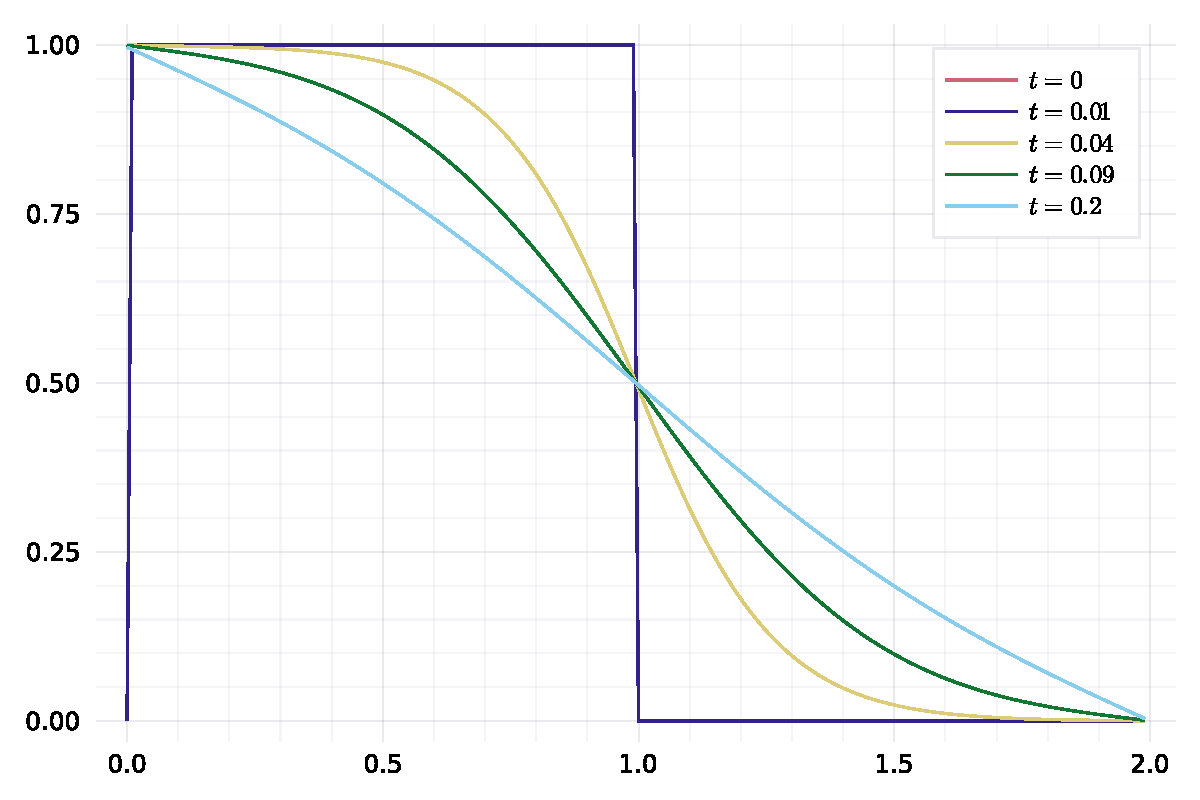
\includegraphics[width=\linewidth]{figures/ass_5_report_5_1.pdf}

\subsection{Crank-Nicolson (CTCS: Trapezoid)}

\begin{lstlisting}
(*@\HLJLn{u}@*) (*@\HLJLoB{=}@*) (*@\HLJLnf{Trapezoid{\_}sys}@*)(*@\HLJLp{(}@*)(*@\HLJLn{M}@*)(*@\HLJLp{,}@*) (*@\HLJLn{T}@*)(*@\HLJLp{,}@*) (*@\HLJLn{u0}@*)(*@\HLJLp{,}@*) (*@\HLJLn{A}@*)(*@\HLJLp{,}@*) (*@\HLJLn{b}@*)(*@\HLJLp{)}@*)

(*@\HLJLcs{{\#}}@*) (*@\HLJLcs{Plotting}@*) (*@\HLJLcs{routine}@*)
(*@\HLJLn{ts}@*) (*@\HLJLoB{=}@*) (*@\HLJLp{(}@*)(*@\HLJLni{1}@*)(*@\HLJLoB{:}@*)(*@\HLJLni{3}@*)(*@\HLJLp{)}@*) (*@\HLJLoB{.{\textasciicircum}}@*)(*@\HLJLni{2}@*) (*@\HLJLoB{*}@*) (*@\HLJLnfB{1e-2}@*)
(*@\HLJLn{ms}@*) (*@\HLJLoB{=}@*) (*@\HLJLn{Int}@*)(*@\HLJLoB{.}@*)(*@\HLJLp{(}@*)(*@\HLJLn{floor}@*)(*@\HLJLoB{.}@*)(*@\HLJLp{((}@*)(*@\HLJLn{ts}@*) (*@\HLJLoB{.-}@*) (*@\HLJLn{t0}@*)(*@\HLJLp{)}@*)(*@\HLJLoB{/}@*)(*@\HLJLn{\ensuremath{\Delta}t}@*)(*@\HLJLp{))}@*)(*@\HLJLcs{{\#}}@*) (*@\HLJLcs{indices}@*) (*@\HLJLcs{for}@*) (*@\HLJLcs{ts}@*)
(*@\HLJLnf{plot}@*)(*@\HLJLp{(}@*)(*@\HLJLn{xs}@*)(*@\HLJLp{[}@*)(*@\HLJLni{1}@*)(*@\HLJLoB{:}@*)(*@\HLJLn{N}@*)(*@\HLJLp{],}@*) (*@\HLJLn{u0}@*)(*@\HLJLp{[}@*)(*@\HLJLni{1}@*)(*@\HLJLoB{:}@*)(*@\HLJLn{N}@*)(*@\HLJLp{],}@*) (*@\HLJLn{label}@*) (*@\HLJLoB{=}@*) (*@\HLJLnf{latexstring}@*)(*@\HLJLp{(}@*)(*@\HLJLs{"{}t}@*) (*@\HLJLs{=}@*) (*@\HLJLs{"{}}@*)(*@\HLJLp{,}@*) (*@\HLJLni{0}@*) (*@\HLJLp{))}@*)
(*@\HLJLn{j}@*) (*@\HLJLoB{=}@*) (*@\HLJLni{1}@*)
(*@\HLJLk{for}@*) (*@\HLJLn{i}@*) (*@\HLJLoB{\ensuremath{\in}}@*) (*@\HLJLn{ms}@*)
    (*@\HLJLnf{plot!}@*)(*@\HLJLp{(}@*)(*@\HLJLn{xs}@*)(*@\HLJLp{[}@*)(*@\HLJLni{1}@*)(*@\HLJLoB{:}@*)(*@\HLJLn{N}@*)(*@\HLJLp{],}@*) (*@\HLJLn{u}@*)(*@\HLJLp{[}@*)(*@\HLJLni{1}@*)(*@\HLJLoB{:}@*)(*@\HLJLn{N}@*)(*@\HLJLp{,}@*) (*@\HLJLn{i}@*)(*@\HLJLp{],}@*) (*@\HLJLn{label}@*) (*@\HLJLoB{=}@*) (*@\HLJLnf{latexstring}@*)(*@\HLJLp{(}@*)(*@\HLJLs{"{}t}@*) (*@\HLJLs{=}@*) (*@\HLJLs{"{}}@*)(*@\HLJLp{,}@*)(*@\HLJLn{ts}@*)(*@\HLJLp{[}@*)(*@\HLJLn{j}@*)(*@\HLJLp{]))}@*)
    (*@\HLJLkd{global}@*) (*@\HLJLn{j}@*) (*@\HLJLoB{=}@*) (*@\HLJLn{j}@*) (*@\HLJLoB{+}@*) (*@\HLJLni{1}@*)
(*@\HLJLk{end}@*)

(*@\HLJLnf{plot!}@*)(*@\HLJLp{(}@*)(*@\HLJLn{xs}@*)(*@\HLJLp{[}@*)(*@\HLJLni{1}@*)(*@\HLJLoB{:}@*)(*@\HLJLn{N}@*)(*@\HLJLp{],}@*) (*@\HLJLn{u}@*)(*@\HLJLp{[}@*)(*@\HLJLni{1}@*)(*@\HLJLoB{:}@*)(*@\HLJLn{N}@*)(*@\HLJLp{,}@*) (*@\HLJLk{end}@*)(*@\HLJLp{],}@*) (*@\HLJLn{label}@*) (*@\HLJLoB{=}@*) (*@\HLJLnf{latexstring}@*)(*@\HLJLp{(}@*)(*@\HLJLs{"{}t}@*) (*@\HLJLs{=}@*) (*@\HLJLs{"{}}@*)(*@\HLJLp{,}@*) (*@\HLJLnfB{0.2}@*)(*@\HLJLp{))}@*)
\end{lstlisting}

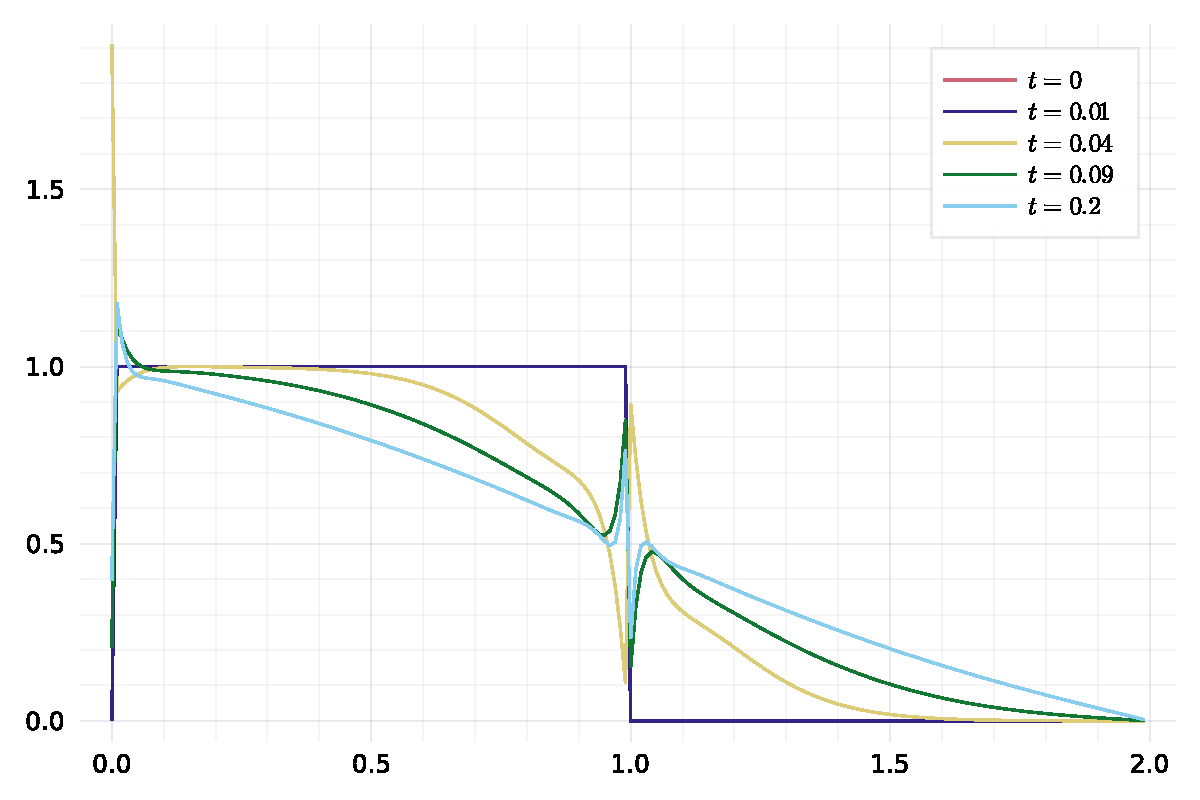
\includegraphics[width=\linewidth]{figures/ass_5_report_6_1.pdf}

\section{Problem 5:}
\subsection{Part 1}

\begin{lstlisting}
(*@\HLJLcs{{\#}}@*) (*@\HLJLcs{Time}@*)
(*@\HLJLn{t0}@*) (*@\HLJLoB{=}@*) (*@\HLJLnfB{0.0}@*)(*@\HLJLp{;}@*) (*@\HLJLn{t}@*) (*@\HLJLoB{=}@*) (*@\HLJLnfB{3.0}@*)(*@\HLJLp{;}@*) 
(*@\HLJLn{T}@*) (*@\HLJLoB{=}@*) (*@\HLJLn{t}@*)(*@\HLJLoB{-}@*)(*@\HLJLn{t0}@*)(*@\HLJLp{;}@*)
(*@\HLJLn{\ensuremath{\Delta}t}@*) (*@\HLJLoB{=}@*) (*@\HLJLnfB{0.01}@*)(*@\HLJLp{;}@*) (*@\HLJLn{M}@*) (*@\HLJLoB{=}@*) (*@\HLJLnf{Int}@*)(*@\HLJLp{(}@*)(*@\HLJLn{T}@*)(*@\HLJLoB{/}@*)(*@\HLJLn{\ensuremath{\Delta}t}@*)(*@\HLJLp{);}@*)

(*@\HLJLcs{{\#}}@*) (*@\HLJLcs{boundary}@*) (*@\HLJLcs{condition}@*)
(*@\HLJLk{function}@*) (*@\HLJLnf{b{\_}}@*)(*@\HLJLp{(}@*)(*@\HLJLn{t}@*)(*@\HLJLp{)}@*)
    (*@\HLJLn{b}@*) (*@\HLJLoB{=}@*) (*@\HLJLnf{zeros}@*)(*@\HLJLp{(}@*)(*@\HLJLn{N}@*)(*@\HLJLp{);}@*)
    (*@\HLJLn{b}@*)(*@\HLJLp{[}@*)(*@\HLJLni{1}@*)(*@\HLJLp{]}@*) (*@\HLJLoB{=}@*) (*@\HLJLnf{cos}@*)(*@\HLJLp{(}@*)(*@\HLJLni{2}@*)(*@\HLJLoB{*}@*)(*@\HLJLn{t}@*)(*@\HLJLp{);}@*)
    (*@\HLJLn{b}@*)(*@\HLJLp{[}@*)(*@\HLJLk{end}@*)(*@\HLJLp{]}@*) (*@\HLJLoB{=}@*) (*@\HLJLnf{sin}@*)(*@\HLJLp{(}@*)(*@\HLJLni{2}@*)(*@\HLJLoB{*}@*)(*@\HLJLn{t}@*)(*@\HLJLp{);}@*)
    (*@\HLJLk{return}@*) (*@\HLJLni{1}@*)(*@\HLJLoB{/}@*)(*@\HLJLp{(}@*)(*@\HLJLn{\ensuremath{\Delta}x}@*)(*@\HLJLoB{{\textasciicircum}}@*)(*@\HLJLni{2}@*)(*@\HLJLp{)}@*) (*@\HLJLoB{*}@*) (*@\HLJLn{b}@*)(*@\HLJLp{;}@*)
(*@\HLJLk{end}@*)

(*@\HLJLn{xs}@*) (*@\HLJLoB{=}@*) (*@\HLJLnf{collect}@*)(*@\HLJLp{(}@*)(*@\HLJLni{0}@*)(*@\HLJLoB{:}@*)(*@\HLJLn{N}@*)(*@\HLJLoB{-}@*)(*@\HLJLni{1}@*)(*@\HLJLp{)}@*)(*@\HLJLoB{*}@*)(*@\HLJLn{\ensuremath{\Delta}x}@*)
(*@\HLJLn{u0}@*) (*@\HLJLoB{=}@*) (*@\HLJLnfB{0.5}@*)(*@\HLJLoB{*}@*)(*@\HLJLnf{f}@*)(*@\HLJLp{(}@*)(*@\HLJLn{xs}@*)(*@\HLJLp{)}@*)

(*@\HLJLcs{{\#}}@*) (*@\HLJLcs{2s}@*) (*@\HLJLcs{DIRK}@*)
(*@\HLJLn{\ensuremath{\alpha}}@*) (*@\HLJLoB{=}@*) (*@\HLJLni{1}@*) (*@\HLJLoB{-}@*) (*@\HLJLni{1}@*)(*@\HLJLoB{/}@*)(*@\HLJLnf{sqrt}@*)(*@\HLJLp{(}@*)(*@\HLJLni{2}@*)(*@\HLJLp{)}@*)
(*@\HLJLn{u}@*) (*@\HLJLoB{=}@*) (*@\HLJLnf{s2{\_}DIRK{\_}sys}@*)(*@\HLJLp{(}@*)(*@\HLJLn{M}@*)(*@\HLJLp{,}@*) (*@\HLJLn{T}@*)(*@\HLJLp{,}@*) (*@\HLJLn{u0}@*)(*@\HLJLp{,}@*) (*@\HLJLn{\ensuremath{\alpha}}@*)(*@\HLJLp{,}@*) (*@\HLJLn{A}@*)(*@\HLJLp{,}@*) (*@\HLJLn{b{\_}}@*)(*@\HLJLp{)}@*)

(*@\HLJLcs{{\#}}@*) (*@\HLJLcs{Plotting}@*) (*@\HLJLcs{routine}@*)
(*@\HLJLn{ts}@*) (*@\HLJLoB{=}@*) (*@\HLJLp{[}@*)(*@\HLJLnfB{0.02}@*)(*@\HLJLp{,}@*)(*@\HLJLnfB{0.5}@*)(*@\HLJLp{,}@*)(*@\HLJLni{1}@*)(*@\HLJLp{]}@*)
(*@\HLJLn{ms}@*) (*@\HLJLoB{=}@*) (*@\HLJLn{Int}@*)(*@\HLJLoB{.}@*)(*@\HLJLp{(}@*)(*@\HLJLn{floor}@*)(*@\HLJLoB{.}@*)(*@\HLJLp{((}@*)(*@\HLJLn{ts}@*) (*@\HLJLoB{.-}@*) (*@\HLJLn{t0}@*)(*@\HLJLp{)}@*)(*@\HLJLoB{/}@*)(*@\HLJLn{\ensuremath{\Delta}t}@*)(*@\HLJLp{))}@*)(*@\HLJLcs{{\#}}@*) (*@\HLJLcs{indices}@*) (*@\HLJLcs{for}@*) (*@\HLJLcs{ts}@*)
(*@\HLJLnf{plot}@*)(*@\HLJLp{(}@*)(*@\HLJLn{xs}@*)(*@\HLJLp{[}@*)(*@\HLJLni{1}@*)(*@\HLJLoB{:}@*)(*@\HLJLn{N}@*)(*@\HLJLp{],}@*) (*@\HLJLn{u0}@*)(*@\HLJLp{[}@*)(*@\HLJLni{1}@*)(*@\HLJLoB{:}@*)(*@\HLJLn{N}@*)(*@\HLJLp{],}@*) (*@\HLJLn{label}@*) (*@\HLJLoB{=}@*) (*@\HLJLnf{latexstring}@*)(*@\HLJLp{(}@*)(*@\HLJLs{"{}t}@*) (*@\HLJLs{=}@*) (*@\HLJLs{"{}}@*)(*@\HLJLp{,}@*) (*@\HLJLni{0}@*) (*@\HLJLp{))}@*)
(*@\HLJLn{j}@*) (*@\HLJLoB{=}@*) (*@\HLJLni{1}@*)
(*@\HLJLk{for}@*) (*@\HLJLn{i}@*) (*@\HLJLoB{\ensuremath{\in}}@*) (*@\HLJLn{ms}@*)
    (*@\HLJLnf{plot!}@*)(*@\HLJLp{(}@*)(*@\HLJLn{xs}@*)(*@\HLJLp{[}@*)(*@\HLJLni{1}@*)(*@\HLJLoB{:}@*)(*@\HLJLn{N}@*)(*@\HLJLp{],}@*) (*@\HLJLn{u}@*)(*@\HLJLp{[}@*)(*@\HLJLni{1}@*)(*@\HLJLoB{:}@*)(*@\HLJLn{N}@*)(*@\HLJLp{,}@*) (*@\HLJLn{i}@*)(*@\HLJLp{],}@*) (*@\HLJLn{label}@*) (*@\HLJLoB{=}@*) (*@\HLJLnf{latexstring}@*)(*@\HLJLp{(}@*)(*@\HLJLs{"{}t}@*) (*@\HLJLs{=}@*) (*@\HLJLs{"{}}@*)(*@\HLJLp{,}@*)(*@\HLJLn{ts}@*)(*@\HLJLp{[}@*)(*@\HLJLn{j}@*)(*@\HLJLp{]))}@*)
    (*@\HLJLkd{global}@*) (*@\HLJLn{j}@*) (*@\HLJLoB{=}@*) (*@\HLJLn{j}@*) (*@\HLJLoB{+}@*) (*@\HLJLni{1}@*)
(*@\HLJLk{end}@*)

(*@\HLJLnf{plot!}@*)(*@\HLJLp{(}@*)(*@\HLJLn{xs}@*)(*@\HLJLp{[}@*)(*@\HLJLni{1}@*)(*@\HLJLoB{:}@*)(*@\HLJLn{N}@*)(*@\HLJLp{],}@*) (*@\HLJLn{u}@*)(*@\HLJLp{[}@*)(*@\HLJLni{1}@*)(*@\HLJLoB{:}@*)(*@\HLJLn{N}@*)(*@\HLJLp{,}@*) (*@\HLJLk{end}@*)(*@\HLJLp{],}@*) (*@\HLJLn{label}@*) (*@\HLJLoB{=}@*) (*@\HLJLnf{latexstring}@*)(*@\HLJLp{(}@*)(*@\HLJLs{"{}t}@*) (*@\HLJLs{=}@*) (*@\HLJLs{"{}}@*)(*@\HLJLp{,}@*) (*@\HLJLnfB{3.0}@*)(*@\HLJLp{))}@*)
\end{lstlisting}

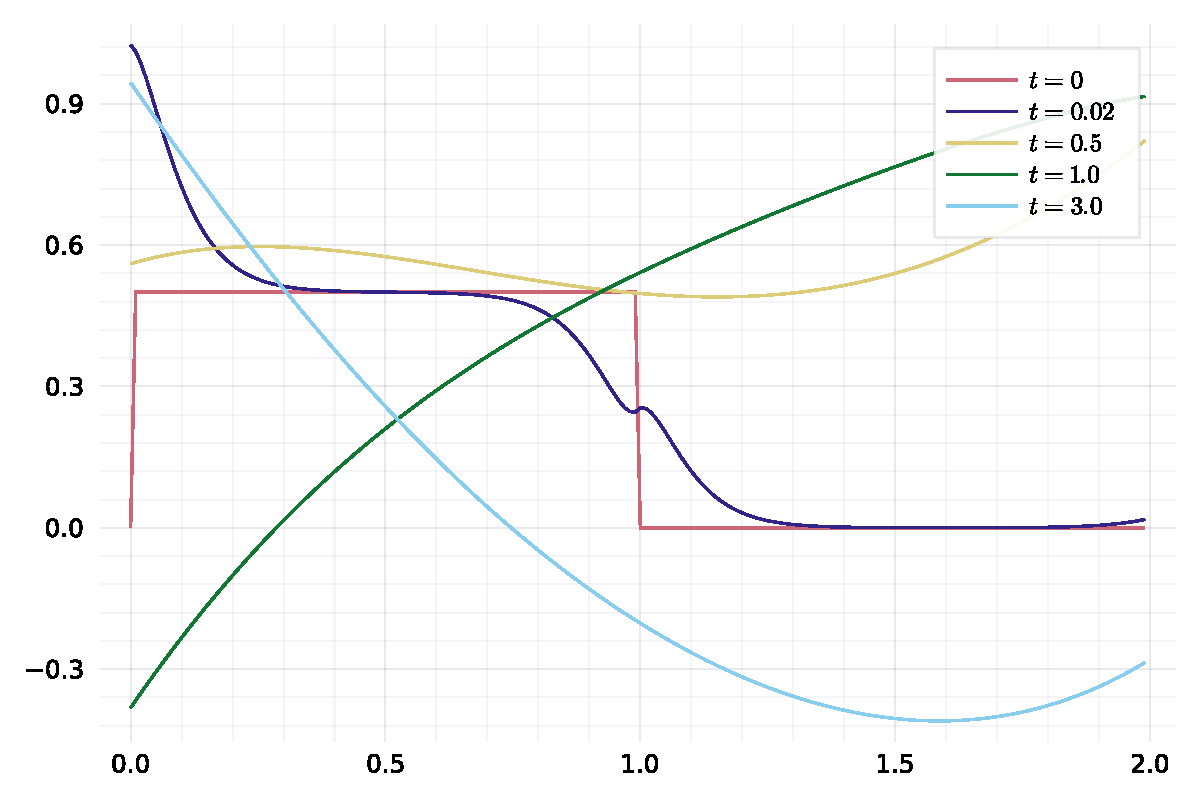
\includegraphics[width=\linewidth]{figures/ass_5_report_7_1.pdf}

\section{Problem 6:}

\begin{lstlisting}
(*@\HLJLcs{{\#}}@*) (*@\HLJLcs{Space}@*)
(*@\HLJLn{x0}@*) (*@\HLJLoB{=}@*) (*@\HLJLnfB{0.0}@*)(*@\HLJLp{;}@*) (*@\HLJLn{x}@*) (*@\HLJLoB{=}@*) (*@\HLJLnfB{2.0}@*)(*@\HLJLp{;}@*)
(*@\HLJLn{N}@*) (*@\HLJLoB{=}@*) (*@\HLJLni{200}@*)(*@\HLJLp{;}@*) (*@\HLJLn{L}@*) (*@\HLJLoB{=}@*) (*@\HLJLn{x}@*)(*@\HLJLoB{-}@*)(*@\HLJLn{x0}@*)(*@\HLJLp{;}@*) (*@\HLJLn{\ensuremath{\Delta}x}@*) (*@\HLJLoB{=}@*) (*@\HLJLn{L}@*)(*@\HLJLoB{/}@*)(*@\HLJLn{N}@*)(*@\HLJLp{;}@*)

(*@\HLJLcs{{\#}}@*) (*@\HLJLcs{Time}@*)
(*@\HLJLn{t0}@*) (*@\HLJLoB{=}@*) (*@\HLJLnfB{0.0}@*)(*@\HLJLp{;}@*) (*@\HLJLn{t}@*) (*@\HLJLoB{=}@*) (*@\HLJLnfB{3.0}@*)(*@\HLJLp{;}@*) 
(*@\HLJLn{T}@*) (*@\HLJLoB{=}@*) (*@\HLJLn{t}@*)(*@\HLJLoB{-}@*)(*@\HLJLn{t0}@*)(*@\HLJLp{;}@*)
(*@\HLJLn{\ensuremath{\Delta}t}@*) (*@\HLJLoB{=}@*) (*@\HLJLnfB{4e-5}@*)(*@\HLJLp{;}@*) (*@\HLJLn{M}@*) (*@\HLJLoB{=}@*) (*@\HLJLnf{Int}@*)(*@\HLJLp{(}@*)(*@\HLJLn{T}@*)(*@\HLJLoB{/}@*)(*@\HLJLn{\ensuremath{\Delta}t}@*)(*@\HLJLp{);}@*)

(*@\HLJLcs{{\#}}@*) (*@\HLJLcs{initial}@*) (*@\HLJLcs{condition}@*)
(*@\HLJLnf{p}@*)(*@\HLJLp{(}@*)(*@\HLJLn{x}@*)(*@\HLJLp{)}@*) (*@\HLJLoB{=}@*) (*@\HLJLp{(}@*)(*@\HLJLni{1}@*) (*@\HLJLoB{.-}@*)(*@\HLJLnfB{0.5}@*)(*@\HLJLoB{*}@*)(*@\HLJLn{x}@*)(*@\HLJLp{)}@*)(*@\HLJLoB{.{\textasciicircum}}@*)(*@\HLJLni{2}@*)

(*@\HLJLcs{{\#}}@*) (*@\HLJLcs{boundary}@*) (*@\HLJLcs{condition}@*)
(*@\HLJLn{\ensuremath{\alpha}}@*) (*@\HLJLoB{=}@*) (*@\HLJLnfB{0.4}@*)
(*@\HLJLnf{q}@*)(*@\HLJLp{(}@*)(*@\HLJLn{t}@*)(*@\HLJLp{)}@*) (*@\HLJLoB{=}@*) (*@\HLJLni{2}@*)(*@\HLJLoB{*}@*)(*@\HLJLnf{sin}@*)(*@\HLJLp{(}@*)(*@\HLJLn{t}@*)(*@\HLJLp{)}@*)(*@\HLJLoB{{\textasciicircum}}@*)(*@\HLJLni{2}@*)
(*@\HLJLn{A}@*) (*@\HLJLoB{=}@*) (*@\HLJLnf{spdiagm}@*)(*@\HLJLp{(}@*)(*@\HLJLoB{-}@*)(*@\HLJLni{1}@*)(*@\HLJLoB{=>}@*)(*@\HLJLnf{ones}@*)(*@\HLJLp{(}@*)(*@\HLJLn{N}@*)(*@\HLJLoB{-}@*)(*@\HLJLni{1}@*)(*@\HLJLp{),}@*)(*@\HLJLni{0}@*)(*@\HLJLoB{=>-}@*)(*@\HLJLnfB{2.0}@*)(*@\HLJLoB{*}@*)(*@\HLJLnf{ones}@*)(*@\HLJLp{(}@*)(*@\HLJLn{N}@*)(*@\HLJLp{),}@*)(*@\HLJLni{1}@*)(*@\HLJLoB{=>}@*)(*@\HLJLnf{ones}@*)(*@\HLJLp{(}@*)(*@\HLJLn{N}@*)(*@\HLJLoB{-}@*)(*@\HLJLni{1}@*)(*@\HLJLp{))}@*)
(*@\HLJLn{A}@*)(*@\HLJLp{[}@*)(*@\HLJLni{1}@*)(*@\HLJLp{,}@*)(*@\HLJLni{1}@*)(*@\HLJLp{]}@*) (*@\HLJLoB{=}@*) (*@\HLJLn{A}@*)(*@\HLJLp{[}@*)(*@\HLJLni{1}@*)(*@\HLJLp{,}@*)(*@\HLJLni{1}@*)(*@\HLJLp{]}@*) (*@\HLJLoB{+}@*) (*@\HLJLp{(}@*)(*@\HLJLni{2}@*)(*@\HLJLoB{-}@*)(*@\HLJLn{\ensuremath{\alpha}}@*)(*@\HLJLoB{*}@*)(*@\HLJLn{\ensuremath{\Delta}x}@*)(*@\HLJLp{)}@*)(*@\HLJLoB{/}@*)(*@\HLJLp{(}@*)(*@\HLJLni{2}@*)(*@\HLJLoB{+}@*)(*@\HLJLn{\ensuremath{\alpha}}@*)(*@\HLJLoB{*}@*)(*@\HLJLn{\ensuremath{\Delta}x}@*)(*@\HLJLp{)}@*)
(*@\HLJLn{A}@*) (*@\HLJLoB{=}@*) (*@\HLJLni{1}@*)(*@\HLJLoB{/}@*)(*@\HLJLp{(}@*)(*@\HLJLn{\ensuremath{\Delta}x}@*)(*@\HLJLoB{{\textasciicircum}}@*)(*@\HLJLni{2}@*)(*@\HLJLp{)}@*)(*@\HLJLoB{*}@*)(*@\HLJLn{A}@*)
(*@\HLJLn{b}@*) (*@\HLJLoB{=}@*) (*@\HLJLnf{zeros}@*)(*@\HLJLp{(}@*)(*@\HLJLn{N}@*)(*@\HLJLp{);}@*) (*@\HLJLn{b}@*)(*@\HLJLp{[}@*)(*@\HLJLk{end}@*)(*@\HLJLp{]}@*) (*@\HLJLoB{=}@*) (*@\HLJLnf{q}@*)(*@\HLJLp{(}@*)(*@\HLJLn{N}@*)(*@\HLJLoB{*}@*)(*@\HLJLn{\ensuremath{\Delta}t}@*)(*@\HLJLp{);}@*) (*@\HLJLn{b}@*) (*@\HLJLoB{=}@*) (*@\HLJLni{1}@*)(*@\HLJLoB{/}@*)(*@\HLJLp{(}@*)(*@\HLJLn{\ensuremath{\Delta}x}@*)(*@\HLJLoB{{\textasciicircum}}@*)(*@\HLJLni{2}@*)(*@\HLJLp{)}@*) (*@\HLJLoB{*}@*) (*@\HLJLn{b}@*)(*@\HLJLp{;}@*)

(*@\HLJLk{function}@*) (*@\HLJLnf{b{\_}}@*)(*@\HLJLp{(}@*)(*@\HLJLn{t}@*)(*@\HLJLp{)}@*)
    (*@\HLJLn{b}@*) (*@\HLJLoB{=}@*) (*@\HLJLnf{zeros}@*)(*@\HLJLp{(}@*)(*@\HLJLn{N}@*)(*@\HLJLp{);}@*) (*@\HLJLn{b}@*)(*@\HLJLp{[}@*)(*@\HLJLk{end}@*)(*@\HLJLp{]}@*) (*@\HLJLoB{=}@*) (*@\HLJLni{2}@*)(*@\HLJLoB{*}@*)(*@\HLJLnf{sin}@*)(*@\HLJLp{(}@*)(*@\HLJLn{t}@*)(*@\HLJLp{)}@*)(*@\HLJLoB{{\textasciicircum}}@*)(*@\HLJLni{2}@*)(*@\HLJLp{;}@*)
    (*@\HLJLk{return}@*) (*@\HLJLni{1}@*)(*@\HLJLoB{/}@*)(*@\HLJLp{(}@*)(*@\HLJLn{\ensuremath{\Delta}x}@*)(*@\HLJLoB{{\textasciicircum}}@*)(*@\HLJLni{2}@*)(*@\HLJLp{)}@*) (*@\HLJLoB{*}@*) (*@\HLJLn{b}@*)(*@\HLJLp{;}@*)
(*@\HLJLk{end}@*)

(*@\HLJLn{xs}@*) (*@\HLJLoB{=}@*) (*@\HLJLnf{collect}@*)(*@\HLJLp{(}@*)(*@\HLJLni{0}@*)(*@\HLJLoB{:}@*)(*@\HLJLn{N}@*)(*@\HLJLoB{-}@*)(*@\HLJLni{1}@*)(*@\HLJLp{)}@*)(*@\HLJLoB{*}@*)(*@\HLJLn{\ensuremath{\Delta}x}@*)
(*@\HLJLn{u0}@*) (*@\HLJLoB{=}@*) (*@\HLJLnf{p}@*)(*@\HLJLp{(}@*)(*@\HLJLn{xs}@*)(*@\HLJLp{)}@*)

(*@\HLJLcs{{\#}}@*) (*@\HLJLcs{FTCS}@*)
(*@\HLJLn{u}@*) (*@\HLJLoB{=}@*) (*@\HLJLnf{ForwardEuler{\_}tsys}@*)(*@\HLJLp{(}@*)(*@\HLJLn{M}@*)(*@\HLJLp{,}@*)(*@\HLJLn{T}@*)(*@\HLJLp{,}@*)(*@\HLJLn{u0}@*)(*@\HLJLp{,}@*)(*@\HLJLn{A}@*)(*@\HLJLp{,}@*)(*@\HLJLn{b{\_}}@*)(*@\HLJLp{)}@*)

(*@\HLJLcs{{\#}}@*) (*@\HLJLcs{Plotting}@*) (*@\HLJLcs{routine}@*)
(*@\HLJLn{ts}@*) (*@\HLJLoB{=}@*) (*@\HLJLp{[}@*)(*@\HLJLnfB{0.02}@*)(*@\HLJLp{,}@*)(*@\HLJLnfB{0.5}@*)(*@\HLJLp{,}@*)(*@\HLJLni{1}@*)(*@\HLJLp{]}@*)
(*@\HLJLn{ms}@*) (*@\HLJLoB{=}@*) (*@\HLJLn{Int}@*)(*@\HLJLoB{.}@*)(*@\HLJLp{(}@*)(*@\HLJLn{floor}@*)(*@\HLJLoB{.}@*)(*@\HLJLp{((}@*)(*@\HLJLn{ts}@*) (*@\HLJLoB{.-}@*) (*@\HLJLn{t0}@*)(*@\HLJLp{)}@*)(*@\HLJLoB{/}@*)(*@\HLJLn{\ensuremath{\Delta}t}@*)(*@\HLJLp{))}@*)(*@\HLJLcs{{\#}}@*) (*@\HLJLcs{indices}@*) (*@\HLJLcs{for}@*) (*@\HLJLcs{ts}@*)
(*@\HLJLnf{plot}@*)(*@\HLJLp{(}@*)(*@\HLJLn{xs}@*)(*@\HLJLp{[}@*)(*@\HLJLni{1}@*)(*@\HLJLoB{:}@*)(*@\HLJLn{N}@*)(*@\HLJLp{],}@*) (*@\HLJLn{u0}@*)(*@\HLJLp{[}@*)(*@\HLJLni{1}@*)(*@\HLJLoB{:}@*)(*@\HLJLn{N}@*)(*@\HLJLp{],}@*) (*@\HLJLn{label}@*) (*@\HLJLoB{=}@*) (*@\HLJLnf{latexstring}@*)(*@\HLJLp{(}@*)(*@\HLJLs{"{}t}@*) (*@\HLJLs{=}@*) (*@\HLJLs{"{}}@*)(*@\HLJLp{,}@*) (*@\HLJLni{0}@*) (*@\HLJLp{))}@*)
(*@\HLJLn{j}@*) (*@\HLJLoB{=}@*) (*@\HLJLni{1}@*)
(*@\HLJLk{for}@*) (*@\HLJLn{i}@*) (*@\HLJLoB{\ensuremath{\in}}@*) (*@\HLJLn{ms}@*)
    (*@\HLJLnf{plot!}@*)(*@\HLJLp{(}@*)(*@\HLJLn{xs}@*)(*@\HLJLp{[}@*)(*@\HLJLni{1}@*)(*@\HLJLoB{:}@*)(*@\HLJLn{N}@*)(*@\HLJLp{],}@*) (*@\HLJLn{u}@*)(*@\HLJLp{[}@*)(*@\HLJLni{1}@*)(*@\HLJLoB{:}@*)(*@\HLJLn{N}@*)(*@\HLJLp{,}@*) (*@\HLJLn{i}@*)(*@\HLJLp{],}@*) (*@\HLJLn{label}@*) (*@\HLJLoB{=}@*) (*@\HLJLnf{latexstring}@*)(*@\HLJLp{(}@*)(*@\HLJLs{"{}t}@*) (*@\HLJLs{=}@*) (*@\HLJLs{"{}}@*)(*@\HLJLp{,}@*)(*@\HLJLn{ts}@*)(*@\HLJLp{[}@*)(*@\HLJLn{j}@*)(*@\HLJLp{]))}@*)
    (*@\HLJLkd{global}@*) (*@\HLJLn{j}@*) (*@\HLJLoB{=}@*) (*@\HLJLn{j}@*) (*@\HLJLoB{+}@*) (*@\HLJLni{1}@*)
(*@\HLJLk{end}@*)

(*@\HLJLnf{plot!}@*)(*@\HLJLp{(}@*)(*@\HLJLn{xs}@*)(*@\HLJLp{[}@*)(*@\HLJLni{1}@*)(*@\HLJLoB{:}@*)(*@\HLJLn{N}@*)(*@\HLJLp{],}@*) (*@\HLJLn{u}@*)(*@\HLJLp{[}@*)(*@\HLJLni{1}@*)(*@\HLJLoB{:}@*)(*@\HLJLn{N}@*)(*@\HLJLp{,}@*) (*@\HLJLk{end}@*)(*@\HLJLp{],}@*) (*@\HLJLn{label}@*) (*@\HLJLoB{=}@*) (*@\HLJLnf{latexstring}@*)(*@\HLJLp{(}@*)(*@\HLJLs{"{}t}@*) (*@\HLJLs{=}@*) (*@\HLJLs{"{}}@*)(*@\HLJLp{,}@*) (*@\HLJLnfB{3.0}@*)(*@\HLJLp{))}@*)
\end{lstlisting}

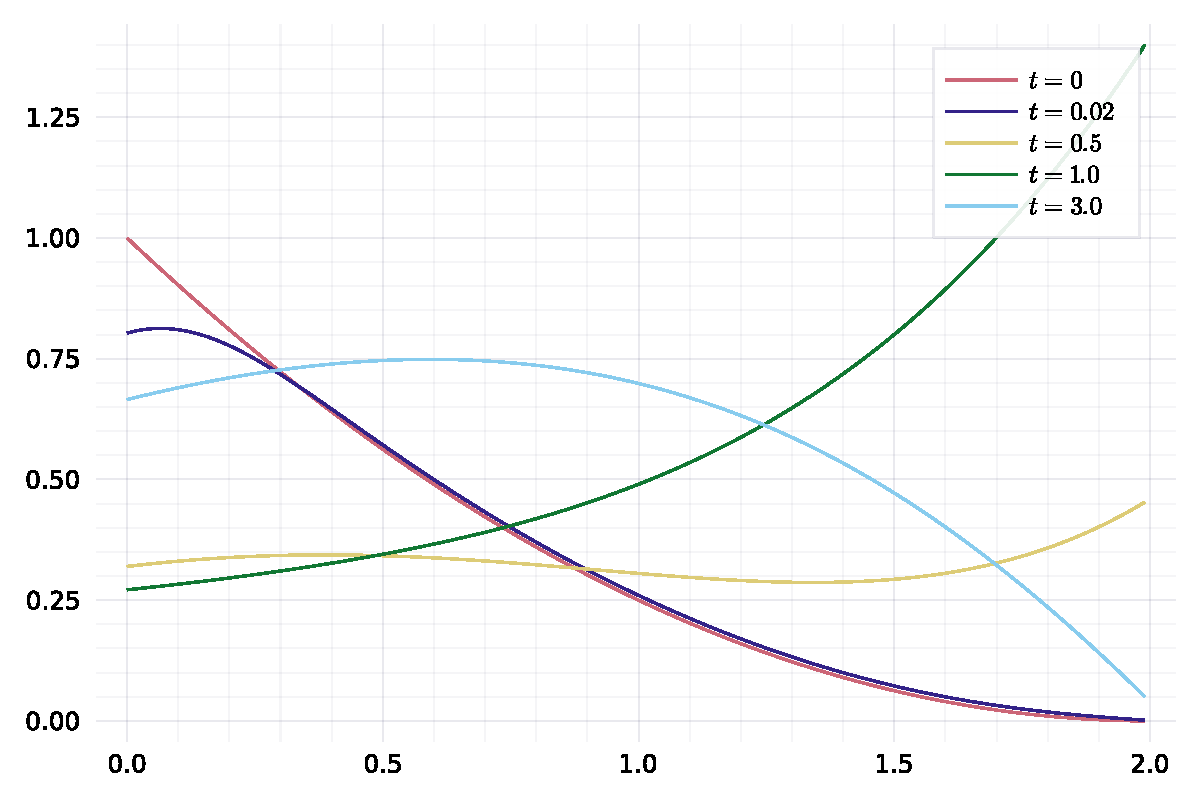
\includegraphics[width=\linewidth]{figures/ass_5_report_8_1.pdf}


\end{document}
